\documentclass[
    english,
    accentcolor=9c,
    design=2023,
    logofile=images/hulogo.pdf,
]{tudabeamer}

\usepackage[english]{babel}
\usepackage[autostyle]{csquotes}
\usepackage{bookmark}
\usepackage[overridenote]{pdfpc}
\usepackage{enumitem}
\usepackage{eurosym}
\usepackage{multirow}
\usepackage{siunitx}

\pdfpcsetup{
    duration=15,
}

\newcommand*{\code}[1]{\texttt{#1}}

\title[LikertShift]{LikertShift - An Input Device for Recording Cycling Subjective Experiences}
\subtitle{Bachelor's Thesis Defense}
\author{Max Schlecht}
\department{Human Computer Interaction}
\institute{Humboldt-Universität zu Berlin}

\date{2025-08-13}

\AtBeginSection{\sectionpage} % Enable section pages

\makeatletter
\patchcmd{\beamer@sectionintoc}
{\vfill}
{\vskip\itemsep}
{}
{}
\makeatother

\let\footnoterule\relax
\renewcommand\thefootnote{}
\setbeamerfont{footnote}{size=\tiny}

\begin{document}

\note{
    - willkommen zur verteidigung meiner bachelorarbeit\\
    - dies das titel und so
}

\maketitle

\note{
    - was ist das Problem das wir loesen wollen\\
    - erklaeren wie der prototyp entworfen und gebaut\\
    - dabei gehe ich kurz auf design requirements, mechanischen aufbau, sowie software ein\\
    - studienplanung zur evaluations\\
    - ergebnisse der studie
}

\tableofcontents

\section{Motivation}

\begin{frame}{Motivation}
    \centering
    \includegraphics[height=0.35\linewidth]{images/vemotion.png}
    \footnotetext{VEmotion (Bethge et al.) \quad \url{https://doi.org/10.1145/3472749.3474775}}

    \note<1>{
        - viele Arbeiten im Human Computer Interaction Berreich die sich mit automatisierter Emotionserkennung z.B. beim Fahren eines Fahrzeuges auseinandersetzen\\
        - die erkannten emotionen koennen z.B. genutzt werden um Sprachassitenten empathischer erscheinen lassen (Sprachton anpassen), Fahrern andere Routen vorschlagen (z.B. langsamere, szenische Route falls nicht in Eile), sogar vom Fahren abhalten (strassenuntauglich)\\
        - grosser Teil der Forschung fokussiert auf Kraftfahrzeuge, da aber vorallem in Grossstaedten das Fahrrad eine immer wichtigere Rolle einnimmt, ist es interessant Forschung auf Radfahrende zu erweitern
    }

    \note<2>{
        - ein vielversprechender Ansatz ist Nutzung vieler verschiedener Kontextinformationen (Mimik, Fahrverhalten, Verkehr, Wetter) -> mit denen Modell trainiert\\
        - dafuer benoetigt man Ground-Truth data\\
        - beim Autofahren einfach -> Mikrofon (Emotionen self reporten)\\
        - geht grundsaetzlich beim Radfahren auch, aber Umgebungsgeraeuche\\
        - alternativ eintragen am Smartphone (nicht waehrend Fahren -> gefaehrlich)\\
        - kam Gedanke verbessern -> haptisch Slider oder so was
    }
\end{frame}

\begin{frame}{Motivation}
    \begin{columns}[onlytextwidth,c]
        \column{.5\linewidth}
        \centering
        \includegraphics[height=0.55\linewidth]{images/button_device.png}
        \footnotetext{Analysis of Overtaking Maneuvers \ldots (L\'{o}pez et al.)}
        \footnotetext{\url{https://doi.org/10.1145/3472749.3474775}}
        \column{.5\linewidth}
        \centering
        \includegraphics<2>[height=0.55\linewidth]{images/brotate.png}
        \footnotetext<2>{Brotate and Tribike \ldots (Wo\'{z}niak et al.)}
        \footnotetext<2>{\url{https://doi.org/10.1145/3472749.3474775}}
    \end{columns}

    \note<1>{
        - gibt es sowas schon?\\
        - spanische Forschungsgruppe hat fuer Studie Box mit mehreren Knoepfen gebaut\\
        - Teilnehmer fahren Landstrasse, bewerten Gefahr Gefuehl wenn ueberholt werden\\
        - simpel, nicht gut zu benutzen, kabel haengen raus -> keine abgeschlossene loesung
    }

    \note<2>{
        - anderer Bereich umgesehen: Arbeit fokussiert Smartphone Eingabegeraete fuers Fahrradfahren\\
        - direkt am griff montiert, ermoeglicht annehmen von anrufen, lautstaerke anpassen etc. (bewegen in beide richtungen + knopf)\\
        - eigentlich einfacher -> was gibts am fahrrad was in mehreren stufen etwas einstellt -> gangschaltung
    }
\end{frame}

\section{Prototype Design}

\begin{frame}{Design Requirements}
    \begin{enumerate}[label=\textsf{DRQ\arabic*}, left=1em .. 4.5em]
        \item<1-> \textbf{Intuitive}

            Using the prototype should be intuitive.

            \note<1>{- Prototyp moeglichst einfach zu benutzen + offensichtlich}

        \item<2-> \textbf{Robust}

            Minimal user intervention and maintenance.

            \note<2>{
                - wartungsarm (Batteriewechsel, langsame Abnutzung)\\
                - Prototyp sollte bei normaler Nutzung nicht kaputt gehen\\
                - in der Lage Umgebungsbedinungen (Regen, Feuchtigkeit, Temperaturschwankungen) auszuhalten
            }

        \item<3-> \textbf{Safe}

            Uncompromising to the user's safety.

            \note<3>{
                - Sicherheit beim Fahrradfahren nicht eingeschraenkt\\
                - gewisse Ablenkung durch Bewerten ist immer gegeben
            }

        \item<4-> \textbf{Affordable}

            Total cost < \euro25.00.

            \note<4>{
                - guenstig, festgelegter maximalpreis von 25 euro\\
                - erschien mit herstellungsmeth., art von hardware erreichbar
            }

        \item<5-> \textbf{Easy to Reproduce}

            Manufactured and assembled with standard components and tools.

            \note<5>{
                - einfach nachzubauen\\
                - benoetigte bauteile + werkzeuge sollten standardmaessig verfuegbar sein
            }
    \end{enumerate}
\end{frame}

\begin{frame}{LikertShift Prototype}
    \begin{columns}[onlytextwidth,c]
        \column{.5\linewidth}
        \centering
        \includegraphics[height=0.7\linewidth]{../images/likertshift_assembled.jpg}
        \column{.5\linewidth}
        \centering
        \includegraphics[height=0.7\linewidth]{../images/likertshift_mounted.jpg}
    \end{columns}
\end{frame}

\begin{frame}{How does it work?}
    \framesubtitle{Mechanics}
    \begin{columns}[onlytextwidth,c]
        \column{.5\linewidth}
        \centering
        \includegraphics[height=0.7\linewidth]{../images/cad_rotator_head.jpg}
        \column{.5\linewidth}
        \centering
        \includegraphics[height=0.7\linewidth]{../images/cad_ramped_track.jpg}
    \end{columns}
\end{frame}

\begin{frame}{How does it work?}
    \framesubtitle{Electronics}
    \begin{columns}[onlytextwidth,c]
        \column{.5\linewidth}
        \centering
        \includegraphics[height=0.7\linewidth]{../images/likertshift_pcb.jpg}
        \column{.5\linewidth}
        \centering
        \includegraphics[height=0.7\linewidth]{../images/cad_pcb_compartment.jpg}
    \end{columns}
\end{frame}

\begin{frame}{How does it work?}
    \framesubtitle{Software}
    \begin{columns}[onlytextwidth,c]
        \column{.25\linewidth}
        \centering
        \includegraphics[height=1.35\linewidth]{../images/app_map_screen.jpg}
        \column{.25\linewidth}
        \centering
        \includegraphics<2->[height=1.35\linewidth]{../images/app_routes_screen.jpg}
        \column{.25\linewidth}
        \centering
        \includegraphics<3->[height=1.35\linewidth]{../images/app_devices_screen.jpg}
        \column{.25\linewidth}
        \centering
        \includegraphics<4->[height=1.35\linewidth]{../images/app_tlx_survey.jpg}
    \end{columns}
\end{frame}

\section{Study Design}

\begin{frame}{Study Design}
    \textbf{What methods are we comparing?}
    \note<1>{
        - was wollen wir ueberhaupt vergleichen?\\
        - verschiedene Methoden zur Messung von CSEs (Subjektive Erfahrungen von Radfahrern)\\
        - Wahl von bereits genutzten Methoden
    }
    \pause

    \quad $\Rightarrow$ \;Audio Recording, Manual Mapping, LikertShift
    \pause

    \vspace*{1em}
    \textbf{What are we measuring?}
    \note<3>{
        - was ist die Metrik die wir Messen wollen?\\
        - zur qualitativen Analyse von Routendaten ist es sinnvoll wenn fuer Studie eine von aeusseren Bedigungen unabhaengige Metrik gewaehlt (Wetter, Verkehr etc.)\\
        - anderseits auch nicht zu einfach (direkte Bewertung vom Untergrund)
    }
    \pause

    \quad $\Rightarrow$ \;Travel Satisfaction, based on the road
    \note<4>{
        - Reisezufriedenheit basierend auf dem Weg\\
        - abhaengig vom Eigenempfinden
    }
    \pause

    \vspace*{1em}
    \textbf{Route Selection}

    \vspace*{1em}
    \footnotesize
    \centering
    \begin{tabular}{c|c|ccccc|c}
        \multirow{2}{*}{Name} & \multirow{2}{2.4em}{Total\newline} & \multicolumn{5}{c|}{Road Type} & \multirow{2}{4.7em}{Number of\newline}\\
        \cline{3-7}
        &&&&&&&\\[-1em]
        & Length & Road & Bike Path & Mixed Path & Pedestrian Way & Other & Crossings\\[0.15em]
        \hline
        &&&&&&&\\[-0.8em]
        North & \SI{2589}{m} &  \SI{191}{m} & \SI{480}{m} & \SI{1135}{m} & \SI{359}{m} & \SI{424}{m} & 13\\[0.3em]
        East  & \SI{2007}{m} &  \SI{853}{m} & \SI{465}{m} &  \SI{173}{m} & \SI{181}{m} & \SI{335}{m} & 9\\[0.3em]
        South & \SI{2289}{m} & \SI{1152}{m} & \SI{677}{m} &  \SI{116}{m} &  \SI{47}{m} & \SI{297}{m} & 9\\
    \end{tabular}
\end{frame}

\begin{frame}{Study Design}
    \framesubtitle{Routes}
    \begin{columns}[onlytextwidth,c]
        \column{.5\linewidth}
        \centering
        \includegraphics[height=0.7\linewidth]{../images/wood_planks_path.jpg}
        \column{.5\linewidth}
        \centering
        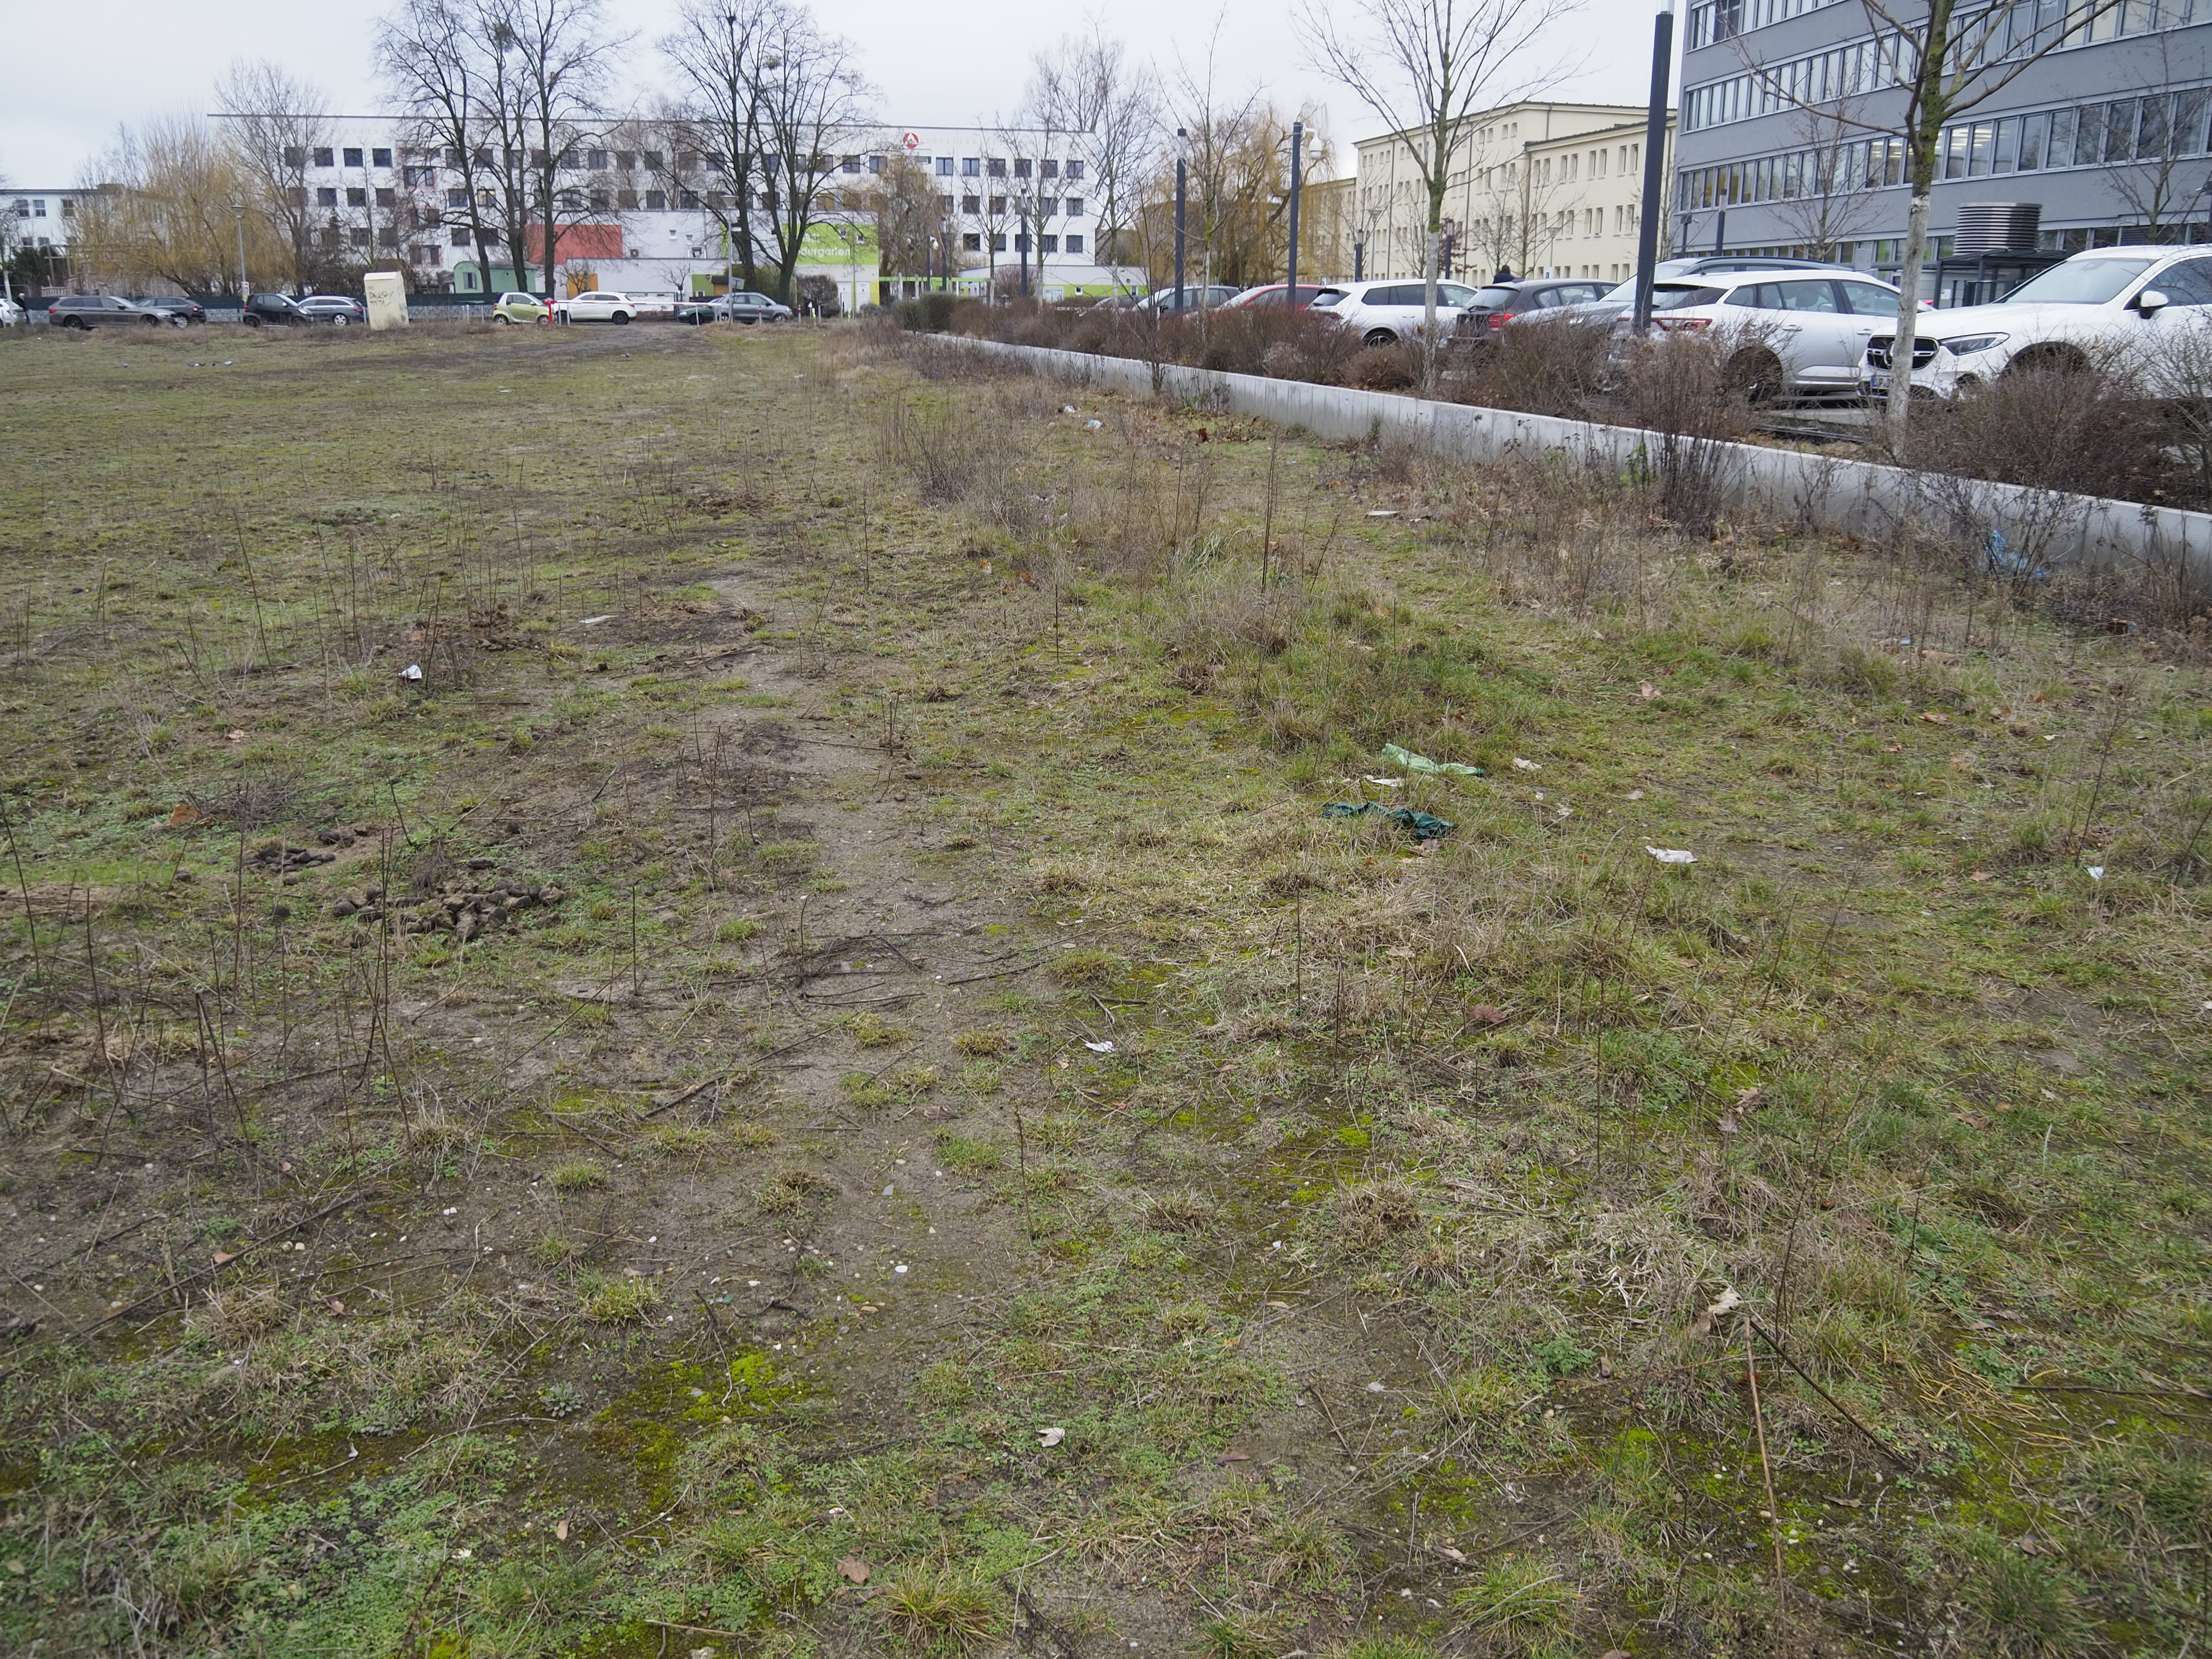
\includegraphics[height=0.7\linewidth]{../images/field_east_route.jpg}
    \end{columns}
\end{frame}

\section{Results}

{
    \setbeamerfont{frametitle}{size=\large}
    \begin{frame}{TLX Results}
        \centering
        \includegraphics[height=0.42\linewidth]{../../evaluation/eval_tlx.pdf}

        \note{
            - Interessant hier Mental Demand, Effort und Frustration weissen Unterschiede mit hoher statistischer Evidenz auf (wo p am geringsten ist)\\
            - auch Interessant: Erwartungen an Performance aehnlich
        }
    \end{frame}
}

{
    \setbeamerfont{frametitle}{size=\large}
    \begin{frame}{UEQ+ Results}
        \centering
        \includegraphics[height=0.42\linewidth]{../../evaluation/eval_ueq.pdf}

        \note{
            - LikertShift besonders attraktiv\\
            - Mapping besondern ineffizient/unintuitiv\\
            - Sicherheitsempfinden aehnlich, Mapping unsicherer wegen hohem Mental Demand (Interviews)\\
            - Social Acceptance von Audio Recording gering, weil unangenehm (auch Bestaetigt in Interviews)
        }
    \end{frame}
}

{
    \setbeamerfont{frametitle}{size=\large}
    \begin{frame}{Recorded Route Data}
        \begin{columns}[onlytextwidth,c]
            \column{.5\linewidth}
            \centering
            \includegraphics[height=0.7\linewidth]{../images/ratings_north_route.jpg}
            \column{.5\linewidth}
            \centering
            \includegraphics[height=0.7\linewidth]{../images/ratings_east_route.jpg}
        \end{columns}
    \end{frame}

    \begin{frame}{Recorded Route Data}
        \begin{table}[!htb]
            \scriptsize
            \centering
            \begin{tabular}{l|ccccccc}
                \multirow{2}{*}{LikertShift} & \multicolumn{7}{c}{Road Type}\\
                \cline{2-8}
                &&&&&&&\\[-1em]
                & Road & Bike Path & Mixed Path & Pedestrian Way & Wood Path & Field & Lawn\\[0.15em]
                \hline
                &&&&&&&\\[-0.8em]
                MEAN     & 3.7661 & 3.4624 & 3.7708 & 3.0176 & 1.8114 & 1.9804 & 2.8664\\[0.3em]
                VARIANCE & 0.9327 & 0.9140 & 0.8548 & 0.8873 & 0.9661 & 1.2512 & 1.3830\\[0.3em]
                STDDEV   & 0.9658 & 0.9560 & 0.9246 & 0.9420 & 0.9829 & 1.1186 & 1.1760\\
            \end{tabular}

            \vspace{1em}
            \begin{tabular}{l|ccccccc}
                \textsf{Audio} & \multicolumn{7}{c}{Road Type}\\
                \cline{2-8}
                &&&&&&&\\[-1em]
                \textsf{Recording} & Road & Bike Path & Mixed Path & Pedestrian Way & Wood Path & Field & Lawn\\[0.15em]
                \hline
                &&&&&&&\\[-0.8em]
                MEAN     & 3.6622 & 3.4978 & 3.7915 & 2.9559 & 2.5513 & 1.6895 & 2.4405\\[0.3em]
                VARIANCE & 0.8519 & 0.7970 & 0.8172 & 1.4158 & 0.5622 & 1.2402 & 0.9290\\[0.3em]
                STDDEV   & 0.9230 & 0.8927 & 0.9040 & 1.1899 & 0.7498 & 1.1137 & 0.9638\\
            \end{tabular}

            \vspace{1em}
            \begin{tabular}{l|ccccccc}
                \multirow{2}{*}{Mapping} & \multicolumn{7}{c}{Road Type}\\
                \cline{2-8}
                &&&&&&&\\[-1em]
                & Road & Bike Path & Mixed Path & Pedestrian Way & Wood Path & Field & Lawn\\[0.15em]
                \hline
                &&&&&&&\\[-0.8em]
                MEAN     & 3.7476 & 3.4952 & 3.7230 & 3.3553 & 2.3586 & 1.0000 & 3.0291\\[0.3em]
                VARIANCE & 0.9192 & 1.0542 & 1.0379 & 1.2773 & 1.5566 & 0.0000 & 1.0891\\[0.3em]
                STDDEV   & 0.9587 & 1.0267 & 1.0188 & 1.1302 & 1.2476 & 0.0000 & 1.0436\\
            \end{tabular}
        \end{table}
    \end{frame}
}

\begin{frame}{Future Work}
    \large

    \vspace*{2em}
    \textbf{Hybrid Methods} - Combination of LikertShift and Mapping Methods
    \pause

    \vspace*{2em}
    \textbf{Improved Feedback} - Sounds / Vibrations
    \pause

    \vspace*{2em}
    \textbf{Software Improvements} - for standalone / long-time Usage Scenarios

    \note<1>{
        - mehrere Teilnehmende in Interviews vorgeschlagen (teils auch nach Fahrt)\\
        - Moeglichkeit aufgenommene Punkte in App verschieben, neue Punkte setzen etc.\\
        - beste von beiden Methoden
    }

    \note<2>{
        - Prototyp rastet nicht optimal auf Stufen ein\\
        - entweder Rastpunkte verbessern, oder Feedback wenn Stufe umgestellt\\
        - z.B. durch Buzzer, Vibrationsmotor\\
        - evtl. verschiedene Patterns fuer Stufen
    }

    \note<3>{
        - Batterielaufzeit ist nicht optimiert\\
        - erfordert teilweise Restrukturierung der Firmware (und App)\\
        - um Daten ueber laengere Zeitraeume (z.B. Monat) aufzunehmen\\
        - Nutzung ganz ohne Smartphone denkbar
    }
\end{frame}

\begin{frame}{Thank you for listening!}
    \large
    \centering

    \vspace*{2.5em}
    \includegraphics[height=0.175\linewidth]{images/github-mark.png}

    \vspace*{1em}
    \textbf{All project sources are available at:}

    \vspace*{0.5em}
    \url{https://github.com/30350n/likertshift}

\end{frame}

\end{document}
